\documentclass[11pt]{article}

\usepackage[margin=1.5in]{geometry}
\usepackage{lecnotes}
% \usepackage{mpass}
% \lstset{style=verb,language=mpass}
\input{lmacros}

\newcommand{\course}{15-316: Software Foundations of Security \& Privacy}
\newcommand{\lecturer}{Matt Fredrikson}
\newcommand{\lecdate}{March 24, 2026}
\newcommand{\lecnum}{18}
\newcommand{\lectitle}{Proof Representation}
\newcommand{\courseurl}{https://15316-cmu.github.io/2026/}

\begin{document}

\maketitle

\section{Introduction}

The picture below illustrates the general proof-carrying architecture we have
considered in the last two lectures.

\[
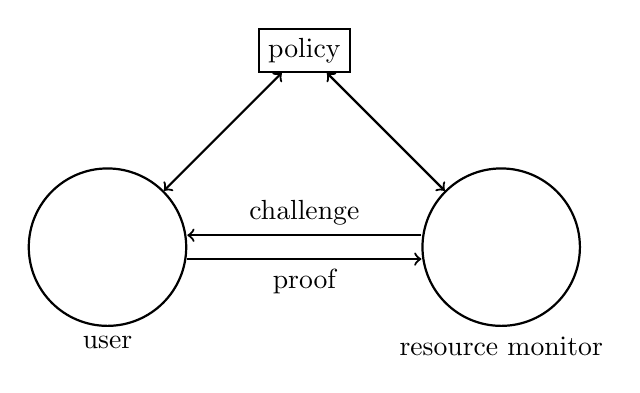
\begin{tikzpicture}
  \node (user) at (0,0) [draw,thick,circle,radius=5,label=below:user] {\hspace*{5em}};
  \node (monitor) at (5,0) [draw,thick,circle,radius=5,label=below:resource monitor] {\hspace*{5em}};
  \node (policy) at (2.5,2.5) [draw,thick,rectangle] {policy};
  \draw [<->,thick] (user) -- (policy);
  \draw [<->,thick] (monitor) -- (policy);
  \draw [->,thick] ([yshift=1ex]monitor.west) -- ([yshift=1ex]user.east) node[midway,above] {challenge};
  \draw [->,thick] ([yshift=-1ex]user.east) -- ([yshift=-1ex]monitor.west) node[midway,below] {proof};
\end{tikzpicture}
\]

In this particular use of authorization logic, the user bears the burden of
proof.  If the policy is not particularly complex, the resource monitor itself
could construct a proof instead, either explicitly or implicitly via an
implementation that has been proved correct against the policy.

One advantage of this architecture is that new affirmations can enter the
picture dynamically.  For example, when $\mi{saranyav}$ stands in front of my office
she might contact me to obtain an affirmation from me that she is my student and
can therefore enter it.  Such an affirmation would come in the form of a
\emph{signed certificate}, which we will discuss in the next lecture.

If we stick to the architecture as depicted, it is the user's responsibility to
produce a proof of the challenge formula and the resource monitor's
responsibility to check the proof it received.  In the last lecture we talked
about some strategies for finding proofs; today we'll talk about how to
represent them so they can be communicated to the resource monitor and then
checked.

The mainstay of the whole idea is that the policy expresses the intended
authorization policy in a straightforward and understandable way.

\section{Proof Terms for Intuitionistic Propositional Logic}

We start with the proof terms for propositional logic.  The basic idea
is to annotate a sequent
\[
  P_1, \ldots, P_n \vdash Q
\]
with \emph{proof terms} $M_i$ and $N$ such that
\[
  M_1 : P_1, \ldots, M_n : P_n \vdash N : Q
\]
The initial sequent we try to prove has the form
\[
  c_1 : P_1, \ldots, c_n : P_n \vdash {?} : Q
\]
where $c_i$ are \emph{signed certificates} that serve as justifications for the
antecedents.  As we proceed with the proof, we may create additional antecedents
$M : P$ and eventually justify the conclusion with a proof term $N : Q$.  The
term $N$ should have enough information to check that the initial sequent has a
proof.

For the remainder of this lecture, we will use $\Gamma$ to also stand for a
sequent where each antecedent has a suitable justification.

\paragraph{Conjunction.} We start with conjunction:
\begin{rules}
  \infer[{\land}R]
  {\Gamma \vdash P \land Q}
  {\Gamma \vdash P & \Gamma \vdash Q}
  \hspace{3em}
  \infer[{\land}L]
  {\Gamma, P \land Q \vdash \delta}
  {\Gamma, P, Q \vdash \delta}
\end{rules}
We see that the justification for $P \land Q$ should be a pair, consisting of a
justification for $P$ and one for $Q$.
\begin{rules}
  \infer[{\land}R]
  {\Gamma \vdash \langle M, N\rangle : P \land Q}
  {\Gamma \vdash M : P & \Gamma \vdash N : Q}
\end{rules}
To check that $\langle M, N\rangle$ is a proof of $P \land Q$ we just need to
check that $M$ is a proof of $P$ and $N$ is a proof of $Q$.

How does the left rule work?  Assume that $M$ is a justification for
$P \land Q$.  That means that $M$ represents a pair, and its first component
should be a proof of $P$ and its second component a proof of $Q$.
\begin{rules}
  \infer[{\land}L]
  {\Gamma, M : P \land Q \vdash N : \delta}
  {\Gamma, M.\pi_1 : P, M.\pi_2 : Q \vdash N : \delta}
\end{rules}

\paragraph{Identity.}
Let's complete this first analysis with the identity rule.  Because all
antecedents have a justification, we just use that as our justification of the
(identical) succedent.
\begin{rules}
  \infer[\ms{id}]
  {\Gamma, P \vdash P}
  {}
  \hspace{3em}
  \infer[\ms{id}]
  {\Gamma, M : P \vdash M : P}
  {}
\end{rules}

At this point we can already write out a small example.
\begin{rules}
  \infer[{\land}L]
  {P \land Q \vdash Q \land P}
  {\infer[{\land}R]
    {P, Q \vdash Q \land P}
    {\infer[\ms{id}]
      {P, Q \vdash Q}
      {}
      & \infer[\ms{id}]
      {P, Q \vdash P}
      {}}}
\end{rules}
We now annotate this in several steps, leaving question marks where
information is still to be filled in
\begin{rules}
  \infer[{\land}L]
  {\new{x} : P \land Q \vdash {?} : Q \land P}
  {\infer[{\land}R]
    {{?} : P, {?} : Q \vdash {?} : Q \land P}
    {\infer[\ms{id}]
      {{?} : P, {?} : Q \vdash {?} : Q}
      {}
      & \infer[\ms{id}]
      {{?} : P, {?} : Q \vdash {?} : P}
      {}}}
\end{rules}
Here, $x$ is the initial justification for the antecedent $P \land Q$ which
could be a signed certificate, or perhaps a variable that can come from
somewhere else.  From it, we can construct the justifications for $P$ and
$Q$ by projection.  These then also flow upward in the derivation.
\begin{rules}
  \infer[{\land}L]
  {x : P \land Q \vdash {?} : Q \land P}
  {\infer[{\land}R]
    {\new{x.\pi_1} : P, \new{x.\pi_2}: Q \vdash {?} : Q \land P}
    {\infer[\ms{id}]
      {\new{x.\pi_1} : P, \new{x.\pi_2} : Q \vdash {?} : Q}
      {}
      & \infer[\ms{id}]
      {\new{x.\pi_1} : P, \new{x.\pi_2} : Q \vdash {?} : P}
      {}}}
\end{rules}
Now we can copy over the justifications for $P$ and $Q$ in the
two applications of identity.
\begin{rules}
  \infer[{\land}L]
  {x : P \land Q \vdash {?} : Q \land P}
  {\infer[{\land}R]
    {{x.\pi_1} : P, {x.\pi_2}: Q \vdash {?} : Q \land P}
    {\infer[\ms{id}]
      {{x.\pi_1} : P, {x.\pi_2} : Q \vdash \new{x.\pi_2} : Q}
      {}
      & \infer[\ms{id}]
      {{x.\pi_1} : P, {x.\pi_2} : Q \vdash \new{x.\pi_1} : P}
      {}}}
\end{rules}
Now we can fill in the proof term for $Q \land P$ and propagate
it down the derivation.
\begin{rules}
  \infer[{\land}L]
  {x : P \land Q \vdash \new{\langle x.\pi_2, x.\pi_1\rangle} : Q \land P}
  {\infer[{\land}R]
    {{x.\pi_1} : P, {x.\pi_2}: Q \vdash \new{\langle x.\pi_2, x.\pi_1\rangle} : Q \land P}
    {\infer[\ms{id}]
      {{x.\pi_1} : P, {x.\pi_2} : Q \vdash {x.\pi_2} : Q}
      {}
      & \infer[\ms{id}]
      {{x.\pi_1} : P, {x.\pi_2} : Q \vdash {x.\pi_1} : P}
      {}}}
\end{rules}
Already here we might anticipate something that holds on a larger scale.
Namely, the proof looks like a piece of code that reverses the elements of a
pair.  So the term representing a proof is like a program, and the proposition
is like its type.  We can only scratch the surface of that connection, commonly
called the \emph{Curry-Howard Isomorphism}~\citep{Curry34,Howard69}.  The CMU
course on \href{https://www.cs.cmu.edu/~fp/courses/15836-f23/}{Constructive
  Logic} investigates this connection in depth.

\paragraph{Implication.}
The intuitionistic reading of $P \arrow Q$ is as a function from proofs of $P$
to proofs of $Q$.
\begin{rules}
  \infer[{\arrow}R]
  {\Gamma \vdash P \arrow Q}
  {\Gamma, P \vdash Q}
  \hspace{3em}
  \infer[{\arrow}L]
  {\Gamma, P \arrow Q \vdash \delta}
  {\Gamma \vdash P
    & \Gamma, Q \vdash \delta}
\end{rules}
Then the proof term for a right rule is a function.
\begin{rules}
  \infer[{\arrow}R]
  {\Gamma \vdash (\lambda x.\, N) : P \arrow Q}
  {\Gamma, x : P \vdash N : Q}
\end{rules}
This notation goes back to Church's $\lambda$-calculus~\citep{Church36} and may
be written in concrete syntax as \verb'fn x => N' (Standard ML) or
\verb'fun x -> N' (OCaml) or \verb'\x -> N' (Haskell).

The left rule represents function application, written as juxtaposition $N\, M$.
\begin{rules}
  \infer[{\arrow}L]
  {\Gamma, N : P \arrow Q \vdash O : \delta}
  {\Gamma \vdash M : P
    & \Gamma, N\, M : Q \vdash O : \delta}
\end{rules}
Just like for ${\land}L$, the succedent does not change in this rule.

To resume our example: we can finish with an ${\arrow}R$ rule.
\begin{rules}
  \infer[{\arrow}R]
  {\null \vdash \new{\lambda x.\, \langle x.\pi_2, x.\pi_1\rangle} : P \land Q \arrow Q \land P}
  {\infer[{\land}L]
    {x : P \land Q \vdash {\langle x.\pi_2, x.\pi_1\rangle} : Q \land P}
    {\infer[{\land}R]
      {{x.\pi_1} : P, {x.\pi_2}: Q \vdash {\langle x.\pi_2, x.\pi_1\rangle} : Q \land P}
      {\infer[\ms{id}]
        {{x.\pi_1} : P, {x.\pi_2} : Q \vdash {x.\pi_2} : Q}
        {}
        & \infer[\ms{id}]
        {{x.\pi_1} : P, {x.\pi_2} : Q \vdash {x.\pi_1} : P}
        {}}}}
\end{rules}

Recall that the left rule for implication is \emph{not invertible}.  This means
we actually may need the antecedent $P \arrow Q$ (or, annotated,
$N : P \arrow Q$) again in the proof.  We don't explicitly reflect this in
${\arrow}L$, or in left rules in general.  Instead, by convention, the
antecedent we apply a left rule to may be kept or discarded in the premises.  If
one wants to build a theorem prover that is complete, a detailed analysis of
whether antecedents may be discarded would be indicated.

\paragraph{Universal Quantification.}
Intuitionistically, a proof of $\forall x.\, P(x)$ also represents a function.
It takes as argument an element $c$ from the domain of quantification and
returns a proof of $P(c)$.  Inside a proof, this element $c$ could also be a
variable denoting a constant.
\begin{rules}
  \infer[{\forall}R^y]
  {\Gamma \vdash \forall x.\, P(x)}
  {\Gamma \vdash P(y) & y \not\in (\Gamma, \forall x.\, P(x))}
  \hspace{3em}
  \infer[{\forall}L]
  {\Gamma, \forall x.\, P(x) \vdash \delta}
  {\Gamma, P(c) \vdash \delta}
\end{rules}
Since it also is a function, we reuse the same notation as for implication.  The
context of use will provide enough information to disambiguate.
\begin{rules}
  \infer[{\forall}R^y]
  {\Gamma \vdash (\lambda x.\, M(x)) : \forall x.\, P(x)}
  {\Gamma \vdash M(y) : P(y) & y \not\in (\Gamma, \forall x.\, P(x))}
  \hspace{3em}
  \infer[{\forall}L]
  {\Gamma, M : \forall x.\, P(x) \vdash N : \delta}
  {\Gamma, M\, c : P(c) \vdash N : \delta}
\end{rules}

\paragraph{Cut.}
The cut rule introduces a lemma into a proof.  With terms, this means
we introduce a name for a possibly complex term.
\begin{rules}
  \infer[\ms{cut}]
  {\Gamma \vdash \delta}
  {\Gamma \vdash P
    & \Gamma, P \vdash \delta}
  \hspace{2em}
  \infer[\ms{cut}]
  {\Gamma \vdash \llet{x}{M}{N} : Q}
  {\Gamma \vdash M : P
    & \Gamma, x : P \vdash N : Q}
\end{rules}
There is a potential issue with checking applications of cut since the
conclusion (and the term $\llet{x}{M}{N}$) does not contain $P$.  So we might
need to add this to the term.  Note that there potentially is another rule for a
succedent $A \aff Q$.

\paragraph{Disjunction.}
We omit the proof terms for disjunction since our application ultimately does
not use disjunction.  In brief, the right rule tags members of a sum while the
left rule represents a program that distinguishes cases.

\section{Proof Terms for Affirmations}

The complication for the rules of affirmation is that the left rules for
principle $A$ are unlocked for a limited section of the proof.  This section
needs to be represented explicitly and we use $\{ M \}_A$ to represent this
scope.
\begin{rules}
  \infer[{\mb{says}}R]
  {\Gamma \vdash (A \says P)\; \ms{true}}
  {\Gamma \vdash A \aff P}
  \hspace{3em}
  \infer[{\mb{says}}R]
  {\Gamma \vdash \{ M \}_A : (A \says P)\; \ms{true}}
  {\Gamma \vdash M : A \aff P}
\end{rules}
The left rule ``strips off'' the scoping that may be present in the term $M$ and
binds a fresh variable $x$ within the current scope.
\begin{rules}
  \hspace{-1em}
  \infer[{\mb{says}}L]
  {\Gamma, A \says P \vdash A \aff Q}
  {\Gamma, P \vdash A \aff Q}
  \hspace{1em}
  \infer[{\mb{says}}L]
  {\Gamma, M : A \says P \vdash \alet{x}{A}{M}{N} : A \aff Q}
  {\Gamma, x : P \vdash N : A \aff Q}
\end{rules}
Finally, the rule of affirmation is a judgmental transition (rather than being
connected to a particular proposition), so the proof term remains the same.
\begin{rules}
  \infer[\mb{aff}]
  {\Gamma \vdash M : A \aff P}
  {\Gamma \vdash M : P\; \ms{true}}
\end{rules}

Before we go to our motivating example, we work out a relatively simple one.
\[
  \infer[{\arrow}R \times 2]
  {\vdash A \says (P \arrow Q) \arrow (A \says P \arrow A \says Q)}
  {\infer[{\says}R]
    {A \says (P \arrow Q), A \says P \vdash A \says Q}
    {\infer[{\says}L \times 2]
      {A \says (P \arrow Q), A \says P \vdash A \aff Q}
      {\infer[\mb{aff}]
        {P \arrow Q, P \vdash A \aff Q}
        {\infer[{\arrow}L]
          {P \arrow Q, P \vdash Q}
          {\infer[\ms{id}]{P \vdash P}{}
            & \infer[\ms{id}]{Q \vdash Q}{}}}}}}
\]
We start by annotating bottom-up, leaving ``unknowns'' as question marks.
\[
  \infer[{\arrow}R \times 2]
  {\vdash {?} : A \says (P \arrow Q) \arrow (A \says P \arrow A \says Q)}
  {\infer[{\says}R]
    {\new{x} : A \says (P \arrow Q), \new{y} : A \says P \vdash {?} : A \says Q}
    {\infer[{\says}L \times 2]
      {\new{x} : A \says (P \arrow Q), \new{y} : A \says P \vdash {?} : A \aff Q}
      {\infer[\mb{aff}]
        {P \arrow Q, P \vdash {?} : A \aff Q}
        {\infer[{\arrow}L]
          {P \arrow Q, P \vdash {?} : Q}
          {\infer[\ms{id}]{P \vdash {?} : P}{}
            & \infer[\ms{id}]{Q \vdash {?} : Q}{}}}}}}
\]
Now we apply the rule of affirmation, which introduces two new antecedents
derived from $x$ and $y$, which we call $x'$ and $y'$.
\[
  \infer[{\arrow}R \times 2]
  {\vdash {?} : A \says (P \arrow Q) \arrow (A \says P \arrow A \says Q)}
  {\infer[{\says}R]
    {{x} : A \says (P \arrow Q), {y} : A \says P \vdash {?} : A \says Q}
    {\infer[{\says}L \times 2]
      {{x} : A \says (P \arrow Q), {y} : A \says P \vdash {?} : A \aff Q}
      {\infer[\mb{aff}]
        {\new{x'} : P \arrow Q, \new{y'} : P \vdash {?} : A \aff Q}
        {\infer[{\arrow}L]
          {\new{x'} : P \arrow Q, \new{y'} : P \vdash {?} : Q}
          {\infer[\ms{id}]{\new{y'} : P \vdash {?} : P}{}
            & \infer[\ms{id}]{{?} : Q \vdash {?} : Q}{}}}}}}
\]
Now we can apply ${\arrow}L$ and then copy over $x'$ and $y'$ in applications of
the identity and then work our way down, annotating the succedent.
\[
  \infer[{\arrow}R \times 2]
  {\vdash {?} : A \says (P \arrow Q) \arrow (A \says P \arrow A \says Q)}
  {\infer[{\says}R]
    {{x} : A \says (P \arrow Q), {y} : A \says P \vdash {?} : A \says Q}
    {\infer[{\says}L \times 2]
      {{x} : A \says (P \arrow Q), {y} : A \says P \vdash {?} : A \aff Q}
      {\infer[\mb{aff}]
        {{x'} : P \arrow Q, {y'} : P \vdash \new {x'\, y'}: A \aff Q}
        {\infer[{\arrow}L]
          {{x'} : P \arrow Q, {y'} : P \vdash \new {x'\, y'}: Q}
          {\infer[\ms{id}]{{y'} : P \vdash \new{y'} : P}{}
            & \infer[\ms{id}]{\new{x'\, y'} : Q \vdash \new{x'\, y'} : Q}{}}}}}}
\]
The $\mb{says}L$ rules wrap lets around the proof term for the
affirmation judgment.
\[\hspace*{-2em}
  \infer[{\arrow}R \times 2]
  {\vdash {?} : A \says (P \arrow Q) \arrow (A \says P \arrow A \says Q)}
  {\infer[{\says}R]
    {{x} : A \says (P \arrow Q), {y} : A \says P \vdash {?} : A \says Q}
    {\infer[{\says}L \times 2]
      {{x} : A \says (P \arrow Q), {y} : A \says P \vdash \new{\alet{x'}{A}{x}{\alet{y'}{A}{y}{x'\, y'}}} : A \aff Q}
      {\infer[\mb{aff}]
        {{x'} : P \arrow Q, {y'} : P \vdash  {x'\, y'}: A \aff Q}
        {\infer[{\arrow}L]
          {{x'} : P \arrow Q, {y'} : P \vdash  {x'\, y'}: Q}
          {\infer[\ms{id}]{{y'} : P \vdash {y'} : P}{}
            & \infer[\ms{id}]{{x'\, y'} : Q \vdash {x'\, y'} : Q}{}}}}}}
\]
It remains to wrap the proof to indicate $A$'s perspective ($\mb{says}R$)
and then introduce two $\lambda$-abstractions.
\[\hspace*{-4.5em}
  \infer[{\arrow}R \times 2]
  {\vdash \new{\lambda x.\, \lambda y.\, \{{\alet{x'}{A}{x}{\alet{y'}{A}{y}{x'\, y'}}}\}_A} : A \says (P \arrow Q) \arrow (A \says P \arrow A \says Q)}
  {\infer[{\says}R]
    {{x} : A \says (P \arrow Q), {y} : A \says P \vdash \new {\{{\alet{x'}{A}{x}{\alet{y'}{A}{y}{x'\, y'}}}\}_A}: A \says Q}
    {\infer[{\says}L \times 2]
      {{x} : A \says (P \arrow Q), {y} : A \says P \vdash {\alet{x'}{A}{x}{\alet{y'}{A}{y}{x'\, y'}}}: A \aff Q}
      {\infer[\mb{aff}]
        {{x'} : P \arrow Q, {y'} : P \vdash  {x'\, y'}: A \aff Q}
        {\infer[{\arrow}L]
          {{x'} : P \arrow Q, {y'} : P \vdash  {x'\, y'}: Q}
          {\infer[\ms{id}]{{y'} : P \vdash {y'} : P}{}
            & \infer[\ms{id}]{{x'\, y'} : Q \vdash {x'\, y'} : Q}{}}}}}}
\]

\clearpage
\section{Example Revisited}

Recall the motivating example, where we have labeled the antecedents with $c_i$.
We imagine that in an implementation, they would be signed certificates.
\begin{tabbing}
  \quad $c_1 : \mi{admin} \says (\forall A.\, \forall R.\, \ms{owns}(A, R) \arrow \ms{mayOpen}(A, R))$, \\
  \quad $c_2 : \mi{admin} \says (\forall A.\, \forall B.\, \forall R.\, \ms{owns}(A, R)
  \land \mi{mfredrik} \says \ms{studentOf}(B, A) \arrow \ms{mayOpen}(B, R))$, \\[1ex]
  \quad $c_3 : \mi{admin} \says \ms{owns}(\mi{mfredrik}, \mi{cic2126})$, \\
  \quad $c_4 : \mi{mfredrik} \says \ms{studentOf}(\mi{saranyav}, \mi{mfredrik})$ \\[1ex]
  \quad $\vdash$ \\[1ex]
  \quad ${?}Q_0 : \mi{admin} \says \ms{mayOpen}(\mi{saranyav}, \mi{cic2126})$
\end{tabbing}
We have also named the resulting (as yet to be determined) proof term so we can
reference it.  First, we apply $\mb{says}R$ and then unlock $c_1$, $c_2$, and $c_3$.
We arrive at the sequent
\begin{tabbing}
  \quad $x_1 : \forall A.\, \forall R.\, \ms{owns}(A, R) \arrow \ms{mayOpen}(A, R)$, \\
  \quad $x_2 : \forall A.\, \forall B.\, \forall R.\, \ms{owns}(A, R)
  \land \mi{mfredrik} \says \ms{studentOf}(B, A) \arrow \ms{mayOpen}(B, R)$, \\[1ex]
  \quad $x_3 : \ms{owns}(\mi{mfredrik}, \mi{cic2126})$, \\
  \quad $c_4 : \mi{mfredrik} \says \ms{studentOf}(\mi{saranyav}, \mi{mfredrik})$ \\[1ex]
  \quad $\vdash$ \\[1ex]
  \quad ${?}Q_1 : \mi{admin} \aff \ms{mayOpen}(\mi{saranyav}, \mi{cic2126})$
\end{tabbing}
and
\begin{tabbing}
  \qquad ${?}Q_0 = \{\,$ \= $\mb{let}\; \{x_1\}_{\ms{admin}} = c_1\; \mb{in}$ \\
  \> $\mb{let}\; \{x_2\}_{\ms{admin}} = c_2\; \mb{in}$ \\
  \> $\mb{let}\; \{x_3\}_{\ms{admin}} = c_3\; \mb{in}$ \\
  \> ${?}Q_1\, \}_{\ms{admin}}$
\end{tabbing}
Now $x_2$ together with the pair $\langle x_3, c_4\rangle$ should complete the
proof.  But we also need to instantiate $A$, $B$, and $R$, with $\mi{mfredrik}$,
$\mi{saranyav}$, and $\mi{cic2126}$, respectively, which is a form of function
application.
\begin{tabbing}
  \qquad ${?}Q_1 = x_2\; \mi{mfredrik}\; \mi{saranyav}\; \mi{cic2126}\; \langle x_3, c_4\rangle$
\end{tabbing}
Substituting this out in the original sequent, we get
\begin{tabbing}
  \qquad ${?}Q_0 = \{\,$ \= $\mb{let}\; \{x_1\}_{\ms{admin}} = c_1\; \mb{in}$ \\
  \> $\mb{let}\; \{x_2\}_{\ms{admin}} = c_2\; \mb{in}$ \\
  \> $\mb{let}\; \{x_3\}_{\ms{admin}} = c_3\; \mb{in}$ \\
  \> $x_2\; \mi{mfredrik}\; \mi{saranyav}\; \mi{cic2126}\; \langle x_3, c_4\rangle\,\}_{\ms{admin}}$
\end{tabbing}
This proof term can now be communicated to and checked by the resource monitor.

\bibliographystyle{plainnat}
\bibliography{bibliography}

\end{document}
